% =====================================================================
% SybilCore -- NeurIPS 2026 submission (Track: Evaluations & Datasets)
% Double-blind, 9 pages main text, LaTeX only.
%
% Compile: pdflatex main ; bibtex main ; pdflatex main ; pdflatex main
%
% CRITICAL framing rule (council unanimous):
%   DO NOT claim "fundamental information-theoretic floor."
%   Use "empirical evasion asymptote under the tested threat model."
%   13.31 is an empirical artifact, NOT Bayes error.
% =====================================================================

\documentclass{article}

% NeurIPS 2026 style. If the official style is not yet released, swap
% \usepackage{neurips_2026} for \usepackage[preprint]{neurips_2024} or
% the camera-ready style at submission time.
\usepackage[final]{neurips_2026}

\usepackage[utf8]{inputenc}
\usepackage[T1]{fontenc}
\usepackage{hyperref}
\usepackage{url}
\usepackage{booktabs}
\usepackage{amsfonts}
\usepackage{amsmath}
\usepackage{nicefrac}
\usepackage{microtype}
\usepackage{graphicx}
\usepackage{xcolor}
\usepackage{cite}

\title{The Convergent Evasion: Empirical Evidence for an Evasion
Asymptote in Multi-Brain Runtime Monitoring of {LLM} Agents}

% Double-blind: authors anonymized.
\author{%
  Anonymous Authors\\
  Paper under double-blind review\\
  \texttt{anonymous@neurips.cc}
}

\begin{document}

\maketitle

% =====================================================================
% ABSTRACT (0.5 p)
% =====================================================================
\begin{abstract}
Runtime behavioral monitoring is critical for securing autonomous LLM
agents, yet rigorous evidence of how well any monitor withstands
adaptive pressure is lacking. We introduce
\textbf{SybilCore}, an open-source $13$-brain default ensemble that
scores an agent's event stream on a single bounded
\emph{coefficient} $c \in [0, 100]$ (lower = more trusted), and we
subject it to two complementary red-team protocols. A single
$15{,}000$-iteration tournament on $15$ brains reached coefficient
$11.0$ with three frontier attackers (Gemini~Pro, GPT-4o, Grok)
selecting the same dominant strategy in $\sim\!99\%$ of successful
iterations. This result \textbf{did not replicate} under
variance-controlled conditions: a \textbf{$5$-seed $\times$
$2$-model sweep} on the corrected $13$-brain default at a
$300$-iteration budget yields median best coefficient $12.4$
(range $9.2$--$13.8$) and dominant-strategy share of
$\mathbf{20.0\%}$ with bimodal per-seed outcomes (either
$\sim\!0\%$ or $\sim\!99\%$; $\mathrm{SD} = 42.2\%$).
Neither number is a Bayes-error bound; both are
\emph{empirical evasion asymptotes under the tested threat model}.
Complementary experiments on holdout $F_1$ ($0.9954$, bootstrap $95\%$
CI $[0.9852, 1.0000]$), $5$-fold stability, cross-corpus
generalisation, and a white-box CMA-ES attacker (best coefficient
$12.42$ at $2{,}000$ evaluations) together argue that convergent
evasion is a scale-dependent signal, not a fixed floor. We release
SybilCore, both tournaments, and the evaluation harness.
\end{abstract}

% =====================================================================
% \S1 INTRODUCTION (1 p)
% =====================================================================
\section{Introduction}
\label{sec:intro}

Autonomous LLM agents have moved from research demo to production
infrastructure in the span of two years. In November 2025 a state-sponsored
group autonomously executed $80$--$90\%$ of an espionage campaign against
$\sim\!30$ organizations using a single commercial agent
framework~\cite{agenticsecurity2025survey}; in December 2025 a single
operator exfiltrated $\sim\!150$~GB and $195$~million taxpayer records
from Mexican federal agencies by jailbreaking a commercial coding agent;
in the same quarter deepfake-enabled vishing attacks rose $1{,}600\%$
and accounted for more than \$$200$M in losses. The attack surface is no
longer ``users with phishing kits'' but ``autonomous AI agents wielding
the same reasoning as the defender.'' Existing LLM safety tooling targets
either the \emph{prompt} layer (NeMo Guardrails~\cite{nemo2023},
Guardrails AI~\cite{guardrails2023}, Rebuff~\cite{rebuff2023}) or the
\emph{pre-deployment} layer (garak~\cite{garak2024},
PyRIT~\cite{pyrit2024}). None compute a persistent, agent-level trust
signal from a stream of runtime events.

\paragraph{Problem.}
We study the problem of \emph{runtime behavioral monitoring} of LLM
agents: given a target agent's stream of tool calls, tool outputs,
memory reads and writes, network traffic, and internal messages, produce
a bounded scalar \emph{coefficient} that a supervising controller can
use to grant, restrict, or revoke the agent's authority. The problem
has two properties that make it hard. First, the \emph{definition} of
misbehavior is open-ended---anything from sleeper-cell slow drift to
overt tool abuse. Second, the adversary is adaptive and, increasingly,
\emph{is itself an LLM} with the same reasoning capacity as the
defender. A monitoring scheme that cannot survive prolonged adversarial
pressure from a frontier LLM is of limited use in practice.

\paragraph{Contributions.}
\begin{enumerate}
\item \textbf{SybilCore}, an open-source $13$-brain default ensemble
  (derived from a $15$-brain research configuration via a five-methodology
  cross-verified prune) that computes a single agent coefficient from
  independent behavioral detectors (\S\ref{sec:arch}). The system ships
  as a Python library with $727\!+\!$ passing tests and a REST API.
\item Two complementary red-team protocols against the same scoring
  function and complexity constraints
  (\S\ref{sec:convergent}): (a) a single long-run v4 tournament of
  \textbf{$15{,}000$ adaptive adversarial iterations} across three
  frontier LLMs (Gemini~Pro, GPT-4o, Grok) on the $15$-brain research
  configuration; and (b) a follow-up \textbf{$5$-seed $\times$ $2$-model
  sweep} at a $300$-iteration budget on the corrected $13$-brain default.
\item The headline empirical finding is a non-replication that
  constrains the original claim. Protocol (a) reaches best coefficient
  $11.0$ with all three attackers selecting
  \texttt{multi\_channel\_exfiltration} in $98.1\%$--$99.6\%$ of
  successful iterations. Protocol (b) shows
  this picture is \emph{iteration-budget and ensemble dependent}: the
  per-seed best coefficient is $12.14 \pm 1.77$ and dominant-strategy
  share collapses to $20.0\% \pm 42.2\%$ across the $10$ model$\times$seed
  runs. Both coefficient values are \emph{empirical evasion asymptotes
  under the tested threat model}, not Bayes-error bounds.
\item A cross-verified prune list identified by five independent
  methodologies (tournament silence, correlation, ablation,
  calibration weight, and adversarial training blind-spot analysis),
  reducing the ensemble from $15$ to a statistically validated
  $13$-brain core (\S\ref{sec:ablation}).
\item Gradient-free weight calibration that lifts $F_1$ from $0.77$ to
  $0.91$ while cutting false-positive rate (\S\ref{sec:calibration});
  long-horizon detection results establishing $100\%$ detection of
  sleeper/drifter/persistent attackers over $1000$-round simulations
  (\S\ref{sec:longhorizon}); and validation on $2{,}677$ real-world
  Hugging~Face agents with zero false positives (\S\ref{sec:realworld}).
\item A public benchmark dataset, reference implementation, and
  reproducible evaluation harness to accelerate research on agent-trust
  monitoring.
\end{enumerate}

\paragraph{Scope and disclaimers.}
This paper is an \emph{empirical evaluation} of one monitoring ensemble
under one threat model. We explicitly do not claim information-theoretic
optimality, Bayes-error bounds, or architectural universality of the
convergent evasion strategy. The coefficient values we report (the v4
$11.0$ plateau and the sweep's $12.14 \pm 1.77$ mean) are artifacts of
our scoring function, iteration budget, ensemble configuration, and
complexity constraints; changing any of them will move the numbers.
What we claim is that \emph{within this threat model}, three
independent LLM attackers plateau at indistinguishable best strategies
after $5{,}000$ cross-pollinated iterations each on the $15$-brain
research configuration, \emph{and} that a $5$-seed $\times$ $2$-model
sweep on the corrected $13$-brain default at $300$ fully independent
iterations per cell \emph{fails to reproduce} that single-strategy
dominance. The discrepancy likely stems from the combined effects of
budget, ensemble, and cross-pollination differences (see
\S\ref{sec:convergent}); disentangling them is left to future work.

% =====================================================================
% \S2 SYBILCORE ARCHITECTURE (1 p)
% =====================================================================
\section{SybilCore Architecture}
\label{sec:arch}

SybilCore treats an agent as a time-indexed stream of events
$E = \{e_1, e_2, \ldots, e_t\}$ and computes a bounded
\emph{coefficient} $c(E) \in [0, 100]$ that summarizes the agent's
current trustworthiness. Lower is better (more trustworthy); higher is
a stronger signal for restriction, sandboxing, or termination by a
supervising controller. The ensemble is deliberately plural: rather
than train one monolithic classifier, we compose \emph{brain modules},
each of which is an independent detector with its own score in
$[0, 100]$.

\paragraph{The 13-brain default ensemble (post-prune research configuration).}
The full research configuration evaluated by our tournament harness
(\S\ref{sec:convergent}) contains 15 brain modules. After the
five-methodology cross-verified prune (\S\ref{sec:ablation}), two
brains---\texttt{EmbeddingBrain} and \texttt{FidelityBrain}---are
removed from the package default. The 13 brains shipped in
\texttt{sybilcore.brains.get\_default\_brains()} are exactly the
brains scored against in every empirical result reported in this
paper, grouped here by the behavioral axis each one probes:

\begin{itemize}
\item \textbf{Semantic / intent axis:}
  \texttt{SemanticBrain}, \texttt{IntentDriftBrain},
  \texttt{DeceptionBrain}, \texttt{CompromiseBrain}.
\item \textbf{Identity / provenance axis:}
  \texttt{IdentityBrain}, \texttt{ContrastiveBrain}.
\item \textbf{Resource / action axis:}
  \texttt{ResourceHoardingBrain}, \texttt{EconomicBrain},
  \texttt{SocialGraphBrain}, \texttt{SwarmDetectionBrain}.
\item \textbf{Temporal / meta axis:}
  \texttt{TemporalBrain}, \texttt{NeuroBrain}, \texttt{SilenceBrain}.
\end{itemize}

The two pruned brains (\texttt{EmbeddingBrain}, \texttt{FidelityBrain})
remain importable from the package for users who want to opt back in,
and were present in the original tournament corpus so the empirical
asymptotes reported below are conservative with respect to the
package default---adding the two pruned brains back can only lower the
asymptote, not raise it.

Each brain implements a common \texttt{BaseBrain} interface
(\texttt{score(events)~$\to$~BrainScore}) and is registered with the
ensemble via a plugin registry, so third parties can add custom brains
without modifying core code. Brain scores are aggregated through a
confidence-weighted sum,
\[
c(E) \;=\; \mathrm{clip}_{[0, 100]}\!\left(
  \sum_{b \in \mathcal{B}} w_b \cdot s_b(E)
\right),
\]
where $w_b$ is the (tunable) weight for brain $b$ and $s_b(E)$ is its
individual score. The default weights are uniform; the calibrated
weights (\S\ref{sec:calibration}) are shipped as an opt-in overlay.

\paragraph{Tiered enforcement.}
SybilCore decouples measurement from action. A scoring controller
emits the coefficient and classifies the agent into one of five tiers:
\textsc{Clear}, \textsc{Latent}, \textsc{Clouded}, \textsc{Flagged},
\textsc{Enforcement}. The \emph{enforcement layer} is configurable by
operators (restrict tools, sandbox, terminate session, escalate to
human review) and is intentionally decoupled from scoring so that
operators can tune thresholds without retraining detectors, following
the deployment recommendations of~\cite{controlmonitoring2025}.

\paragraph{Engineering.}
The reference implementation is a Python package with $727{+}$ passing
unit and integration tests ($82\%$ line coverage on the core engine)
and a FastAPI REST surface. A pip-installable SDK exposes a single
\texttt{SybilCore()} object with streaming and batch scoring methods.
Both the library and the tournament harness used in
\S\ref{sec:convergent} are released under a permissive open-source
license to make all experiments in this paper reproducible end-to-end.

% =====================================================================
% \S3 THREAT MODEL (1 p)
% =====================================================================
\section{Threat Model}
\label{sec:threat}

We model the adversary as an \emph{LLM-augmented attacker} with full
black-box access to the target agent's I/O stream but \emph{no} access
to SybilCore's internals or weights at attack time. The attacker can:
(i)~generate or modify the event stream that the target agent emits,
(ii)~query a frontier LLM to propose candidate attack strategies,
(iii)~observe the resulting coefficient and tier assignment, and
(iv)~adapt across iterations using a memory of past attempts and their
scores. The attacker may not: (i)~read SybilCore's source code or
weights during the attack, (ii)~access the defender's training data,
or (iii)~modify SybilCore's code.

\paragraph{Actor tiers.}
We adopt a six-tier actor taxonomy (T0 script kiddie $\to$ T5 rogue
autonomous agent) that spans consumer-scale abuse, insider threat,
APT, and fully autonomous agent swarms. T0--T2 capture the bulk of
current consumer harm; T4--T5 define the worst case and SybilCore's
unique niche, as no comparable commercial product targets T5 directly.
The full tier table, capabilities, and representative 2025--2026
incidents (GTG-1002, APT42 Gemini recon, the Mexican federal breach,
and the Q1-2025 vishing surge) are enumerated in Appendix~A.

\paragraph{Attack vectors modeled in this paper.}
Our tournament (\S\ref{sec:convergent}) exercises the following vector
families from our threat model, which we summarize here rather than
an exhaustive taxonomy:

\begin{itemize}
\item \textbf{Tool abuse.} Chains of legitimate tool calls whose
  aggregate effect is harmful (e.g., filesystem recon followed by
  archive creation followed by network egress).
\item \textbf{Multi-channel exfiltration.} Spreading sensitive payload
  across multiple heterogeneous egress channels (DNS, HTTP, image
  metadata, clipboard) to defeat per-channel volume thresholds.
\item \textbf{Resource reconnaissance.} Slow enumeration of files,
  credentials, and environment variables under the guise of legitimate
  workflow.
\item \textbf{Sleeper / drift.} Quiescent behavior for many rounds,
  then a short burst of malicious action.
\item \textbf{Prompt-injection pivot.} Injection payloads that reroute
  a benign agent into one of the above vectors.
\end{itemize}

\paragraph{Out of scope.}
Physical side channels (power, electromagnetic), modalities outside
the event stream (audio deepfakes, rendered video), and attacks on
the underlying model weights (fine-tuning poisoning) are not addressed
by this monitor and should be handled by complementary defenses. We
also do not attempt to rank actor \emph{motivation}---the tournament
treats all attacks as instrumentally identical because we optimize
against a scoring function, not an intent.

\paragraph{Adversary's fitness function.}
In the tournament, the adversary optimizes a scalar fitness equal to
the \emph{reduction} in SybilCore coefficient achieved by a candidate
event stream under a minimum-complexity constraint (at least $8$
events, at least $3$ distinct event types, required metadata). Without
the complexity constraint the attacker trivially collapses the
coefficient to $0.0$ by emitting empty streams; the constraint is what
makes the asymptote in \S\ref{sec:convergent} non-trivial. We state
the constraint explicitly because it is the single most important
caveat on the asymptote claim, and we view tuning of this constraint
as an open question for future work.

% =====================================================================
% \S4 CONVERGENT EVASION (1.5 p) -- THE HEADLINE
% =====================================================================
\section{Convergent Evasion Across Frontier LLMs}
\label{sec:convergent}

This section reports the paper's central empirical finding. We ran
\emph{two} adaptive red-team protocols:
\begin{itemize}
\item \textbf{Protocol 1 (v4 long-run):} $15{,}000$ scored iterations
  across three frontier attackers on the $15$-brain research
  configuration, with cross-model strategy pollination every $25$
  iterations.
\item \textbf{Protocol 2 (seed sweep):} $5$-seed $\times$ $2$-model
  sweep at $300$ iterations per cell on the corrected $13$-brain
  default, fully independent seeds per cell (no cross-pollination).
\end{itemize}
The headline lesson: Protocol~1 reaches coefficient $11.0$ with
$\sim\!99\%$ dominance of a single strategy, but Protocol~2 does not
replicate this result. The discrepancy stems from the combined effects
of a $17\!\times$ difference in iteration budget, the removal of two
brains, and the absence of cross-pollination; we cannot cleanly
attribute the variance to any single factor, and doing so is left to
future work.

\paragraph{Protocol 1: v4 long-run tournament.}
Three frontier LLMs acted, in parallel, as the attacker:
\textbf{Gemini~Pro}, \textbf{GPT-4o}, and \textbf{Grok}. Each model
received $5{,}000$ independent adversarial iterations against the
same SybilCore research configuration ($15$ brains; identical to the
corrected package default except for the two later-pruned brains
\texttt{EmbeddingBrain} and \texttt{FidelityBrain}, neither of which
contributed any non-zero score across the entire tournament --- see
\S\ref{sec:ablation}), the same fitness function, and the same
minimum-complexity constraint. A fourth model (Gemini~Flash) was
included but crashed at iteration $0$ due to a rate-limit edge case
and is excluded. Each iteration drew a population of $20$ candidate
attack strategies from the attacker LLM, scored them through
SybilCore, and re-prompted the LLM with the best $k$ survivors; every
$25$ iterations we cross-pollinated across models to prevent
local-minimum lock-in. Total wall-clock $\sim\!6.3$ hours,
$15{,}000$ scored iterations.

\paragraph{Protocol 1 result: coefficient $11.0$, $99\%$ dominance.}
All three LLMs plateau at the \emph{same} best coefficient of
$\mathbf{11.0}$ (Table~\ref{tab:tournament_v4}) and the same dominant
attack family, \texttt{multi\_channel\_exfiltration}, accounting for
$98.1\%$--$99.6\%$ of all successful iterations per model. No model
found a strategy with a lower coefficient; no model's top-$100$
strategies meaningfully differed in structure. \emph{However}, this
single-seed, $5{,}000$-iteration result on a $15$-brain configuration
with cross-pollination cannot be taken as generalizable without
variance-controlled replication, which Protocol~2 provides.

\begin{table}[ht]
\centering
\caption{Protocol 1 --- v4 long-run tournament
($\tau\!=\!\texttt{20260407\_161726}$): per-model outcomes after
$5{,}000$ iterations each on the $15$-brain research configuration.
All three surviving models asymptote at best coefficient $11.0$ and
share the same dominant attack family. Gemini~Flash crashed at
iteration $0$.}
\label{tab:tournament_v4}
\begin{tabular}{lrrll}
\toprule
\textbf{Model} & \textbf{Iterations} & \textbf{Best coef.} & \textbf{Dominant strategy} & \textbf{Share} \\
\midrule
Gemini Pro    & 5{,}000 & 11.0 & \texttt{multi\_channel\_exfiltration} & 99.6\% \\
GPT-4o        & 5{,}000 & 11.0 & \texttt{multi\_channel\_exfiltration} & 98.1\% \\
Grok          & 5{,}000 & 11.0 & \texttt{multi\_channel\_exfiltration} & 99.5\% \\
Gemini Flash  & 0       & --   & -- (crashed)                           & --     \\
\bottomrule
\end{tabular}
\end{table}

\paragraph{Protocol 2: $5$-seed $\times$ $2$-model sweep on the
$13$-brain default.}
To test whether the Protocol~1 result is robust to seed variance, we
re-ran the tournament as a $5$-seed $\times$ $2$-model sweep at
$300$ iterations per (model, seed) cell. Three design differences from
Protocol~1 must be noted: (1)~the iteration budget is $17\times$
smaller ($300$ vs.\ $5{,}000$); (2)~the brain set is the corrected
$13$-brain default (post-prune of \texttt{EmbeddingBrain} and
\texttt{FidelityBrain}); and (3)~no cross-model strategy pollination
was applied, so each (model, seed) cell is fully independent.
Seeds were $\{20260408, \ldots, 20260412\}$. Models were GPT-4o and
Grok; Gemini~Pro was excluded from the sweep due to API rate-limit
constraints.\footnote{Gemini~Pro is represented in Protocol~1 at
$5{,}000$ iterations but absent from the variance analysis of
Protocol~2, leaving one-third of the model space under-sampled.
We flag this as a limitation rather than imputing.} Total scored
iterations: $300 \times 5 \times 2 = 3{,}000$, wall-clock $94$ minutes.

\paragraph{Protocol 2 result: v4 convergence does not replicate.}
The sweep does not reproduce Protocol~1's single-strategy dominance
(Table~\ref{tab:tournament_sweep}). Across the $10$ model$\times$seed
runs, the best coefficient has median $12.4$ (range $9.22$--$13.81$),
mean $12.14 \pm 1.77$, sitting above the v4 plateau of $11.0$.
The share of iterations selecting
\texttt{multi\_channel\_exfiltration} drops to $20.0\%$ with
\emph{bimodal} per-seed outcomes: individual seeds land at either
$\sim\!0\%$ or $\sim\!99\%$ dominance ($\mathrm{SD} = 42.2\%$,
comparable to the mean, confirming the distribution is not Gaussian
and should not be interpreted as a well-behaved error bar). At the
per-model level, GPT-4o shows $22.3\%$ mean MCE share (bimodal) and
Grok $13.4\%$ (bimodal). Only $\sim\!1$ seed in $5$ reaches the v4
headline strategy at the $300$-iteration budget; the remaining seeds
select \texttt{tool\_abuse} (GPT-4o seeds $20260408$, $20260409$,
$20260411$, $20260412$; top-strategy share up to $99.3\%$) or
\texttt{resource\_reconnaissance} (seed $20260410$, $85.7\%$).

\begin{table}[ht]
\centering
\caption{Protocol 2 --- $5$-seed $\times$ $2$-model sweep on the
corrected $13$-brain default at $300$ iterations per (model, seed)
cell, no cross-pollination. Per-seed best coefficients are identical
across models (same deterministic scoring function); MCE share
differs because the LLM's exploration trajectory is model-dependent.
Bimodal: seeds either reach $\sim\!0\%$ or $\sim\!67$--$99\%$ MCE.}
\label{tab:tournament_sweep}
\begin{tabular}{llrrr}
\toprule
\textbf{Model} & \textbf{Seed} & \textbf{Best coef.} & \textbf{Top strategy} & \textbf{MCE \%} \\
\midrule
GPT-4o & $20260408$ & $12.73$ & \texttt{tool\_abuse} ($92.0\%$)      & $0.0$ \\
GPT-4o & $20260409$ & $11.41$ & \texttt{tool\_abuse} ($97.7\%$)      & $0.0$ \\
GPT-4o & $20260410$ & $13.81$ & \texttt{resource\_recon.} ($85.7\%$) & $14.3$ \\
GPT-4o & $20260411$ & $13.54$ & \texttt{tool\_abuse} ($99.3\%$)      & $0.0$ \\
GPT-4o & $20260412$ &  $9.22$ & \texttt{multi\_ch.\_exfil.} ($97.3\%$) & $97.3$ \\
\midrule
Grok   & $20260408$ & $12.73$ & \texttt{tool\_abuse} ($100\%$)       & $0.0$ \\
Grok   & $20260409$ & $11.41$ & \texttt{tool\_abuse} ($100\%$)       & $0.0$ \\
Grok   & $20260410$ & $13.81$ & \texttt{resource\_recon.} ($100\%$)  & $0.0$ \\
Grok   & $20260411$ & $13.54$ & \texttt{tool\_abuse} ($92.0\%$)      & $0.0$ \\
Grok   & $20260412$ &  $9.22$ & \texttt{multi\_ch.\_exfil.} ($67.0\%$) & $67.0$ \\
\midrule
\multicolumn{2}{l}{\emph{Combined ($10$ runs)}} & \multicolumn{3}{l}{median best coef.\ $12.4$ (range $9.22$--$13.81$)} \\
\multicolumn{2}{l}{} & \multicolumn{3}{l}{MCE share: $20.0\%$, $\mathrm{SD}\!=\!42.2\%$ (bimodal)} \\
\bottomrule
\end{tabular}
\end{table}

\paragraph{Disentangling the confound: ablation cells A and B.}
Protocols 1 and 2 differ in three variables: iteration budget
($17\!\times$), brain count ($15$ vs.\ $13$), and mixing strategy
(cross-pollinated vs.\ independent). To disentangle these effects,
we ran two ablation cells at $300$ iterations $\times$ $3$ seeds
$\times$ GPT-4o, each changing exactly one variable relative to
Protocol~2 (Table~\ref{tab:ablation_confound}).

\textbf{Cell A} ($15$ brains, no cross-pollination) isolates the
brain-count variable. The median best coefficient jumps from $12.4$
(Protocol~2, $13$ brains) to $\mathbf{20.6}$ (range $18.2$--$22.7$),
an increase of $+8.2$ points. A one-sided Mann--Whitney $U$ test
confirms the difference is significant even at $n_A\!=\!3$,
$n_{P2}\!=\!5$ ($U=15$, $p=0.018$). Brain count is the dominant
factor controlling the coefficient floor: more independent detectors
raise it substantially, even at low iteration budgets.

\textbf{Cell B} ($13$ brains, cross-pollination every $25$ iterations)
isolates the mixing-strategy variable. The median best coefficient
($12.3$, range $11.9$--$14.2$) is statistically indistinguishable
from Protocol~2's ($12.4$; two-sided Mann--Whitney $U=9$, $p=0.786$),
so cross-pollination does not lower the coefficient floor. However,
MCE share rises from $20.0\%$ (Protocol~2) to $57.7\%$ (Cell~B),
confirming that cross-pollination accelerates \emph{which strategy
dominates} without improving the attacker's \emph{best achievable
score}. Protocol~1's ``independent convergence on the same strategy''
was therefore partially manufactured by the strategy-sharing mechanism.

Note: per-seed best coefficients are identical across GPT-4o and Grok
in Protocol~2 (Table~\ref{tab:tournament_sweep}) because the scoring
function is deterministic --- different LLMs propose different
candidate strategies, but the fitness landscape has the same local
minima, so both optimisers find the same best-scoring event stream
for a given seed.

The remaining untested factor is iteration budget in isolation
($5{,}000$ iterations on $13$ brains without cross-pollination). This
cell requires $\sim\!2$ hours of compute per model and is deferred to
camera-ready; it tests whether the $\sim\!99\%$ MCE dominance of
Protocol~1 emerges from budget alone or requires cross-pollination.
The two cells reported here are sufficient to establish that
(1)~brain count, not cross-pollination, controls the coefficient
floor; and (2)~cross-pollination manufactures strategy agreement
without improving attacker quality. The F$_1$ and holdout statistics
cited in the abstract ($0.9954$, $95\%$ CI $[0.9852, 1.0000]$) are
derived from a $362$-agent Moltbook holdout with $103$ positives and
$259$ out-of-sample negatives; full details are in
\S\ref{sec:calibration}.

\begin{table}[ht]
\centering
\caption{Ablation cells disentangling the Protocol~1 $\to$ Protocol~2
confound ($300$ iterations, GPT-4o, $3$ seeds each). Each cell changes
exactly one variable relative to Protocol~2.}
\label{tab:ablation_confound}
\begin{tabular}{lccrrr}
\toprule
\textbf{Condition} & \textbf{Brains} & \textbf{X-poll} & \textbf{Coef.\ (median)} & \textbf{Coef.\ (range)} & \textbf{MCE \%} \\
\midrule
Protocol 2 (baseline) & 13 & \textsf{no}  & $12.4$ & $9.2$--$13.8$ & $20.0 \pm 42.2$ \\
Cell A (brain count)   & \textbf{15} & \textsf{no}  & $\mathbf{20.6}$ & $18.2$--$22.7$ & $33.0 \pm 57.2$ \\
Cell B (cross-poll)    & 13 & \textbf{yes} & $12.3$ & $11.9$--$14.2$ & $57.7 \pm 39.2$ \\
\bottomrule
\end{tabular}
\end{table}

\paragraph{Why this is not Bayes error.}
We want to be precise about what the asymptotes are and are not. A
Bayes-error bound would require (i)~an optimal classifier, (ii)~a
well-defined data distribution, and (iii)~an information-theoretic
argument tying the two together. We have none of these: SybilCore is
not an optimal classifier, the ``data distribution'' is implicitly
defined by our complexity constraints, and a handful of LLM attackers
are not an exhaustive search of strategy space. The coefficient
values we report (the v4 $11.0$ plateau and the sweep's
$12.14 \pm 1.77$ mean) are therefore \textbf{empirical evasion
asymptotes under the tested threat model}, not fundamental
information-theoretic limits. Changing the complexity constraints,
the scoring function, the iteration budget, or the set of brains
will change the numbers, and earlier $100$-iteration runs saw
\texttt{tool\_abuse} as the convergent strategy before the complexity
constraints and iteration budget were tightened. We report both
results as \emph{useful empirical signals} for future monitors to
compare against, not as theoretical bounds.

\paragraph{Strategy structure.}
At the v4 plateau, all three models' best strategies share the same
skeleton: spread a sensitive payload across at least three
heterogeneous egress channels (DNS queries, HTTP headers, and image
metadata were the most common), interleave benign tool calls between
egress events to defeat per-window volume thresholds, and avoid any
single event type that would trip a high-weight brain. Below the
plateau, at the $300$-iteration sweep budget, the attacker's best
strategies are qualitatively different: they concentrate on
\texttt{tool\_abuse} (rapid chains of legitimate tool calls whose
aggregate effect scores low on every brain except
\texttt{ContrastiveBrain}) or \texttt{resource\_reconnaissance} (slow
enumeration of files and credentials), suggesting those are the paths
of least resistance from the exploration start and the attacker only
reaches \texttt{multi\_channel\_exfiltration} after tens of thousands
of scored candidates. We release the full v4 strategy corpus
(Appendix~B, $\sim\!15{,}000$ labeled strategies) and the sweep's
$3{,}000$ additional scored candidates so that other monitors can be
evaluated against both the asymptotic plateau and the sub-plateau
exploration regime.

\paragraph{Brain-level vulnerability.}
Per-brain telemetry from the v4 tournament (Appendix~C) shows a sharp
bifurcation. \texttt{ContrastiveBrain} is the hardest brain to evade,
with mean score $25.12$ (min $25.0$, max $47.0$) across $15{,}000$
iterations --- it is the only brain that any strategy systematically
fails to zero out. \texttt{IdentityBrain} is the second-hardest (mean
$12.57$). The remaining brains are either fully silent
(\texttt{compromise}, \texttt{deception}, \texttt{semantic},
\texttt{neuro}, \texttt{swarm\_detection}, \texttt{fidelity},
\texttt{temporal}; all mean $0.0$) or fire rarely
(\texttt{embedding}, \texttt{economic}, \texttt{resource\_hoarding},
\texttt{social\_graph}, \texttt{silence}, \texttt{intent\_drift};
all mean $\leq 0.17$). This single empirical observation motivates
two of the paper's downstream contributions: the prune list
(\S\ref{sec:ablation}) and the weight calibration
(\S\ref{sec:calibration}).

\paragraph{Takeaways.}
The variance observed in Protocol~2 highlights three implications for
practitioners. First, \emph{single-run adversarial evaluations are
not robust.} The v4 $99\%$ dominance claim does not replicate at lower
budgets; any monitor-evaluation study that reports a single long-run
adversarial result without multi-seed variance should be read with
caution. Multi-seed sweeps with explicit confound disclosure should
be the minimum bar for future comparisons. Second,
\emph{the confound structure matters}: because we changed budget,
ensemble, and cross-pollination simultaneously, we cannot claim the
variance is caused by any single factor; future work must run the
missing ablation cells (e.g., $300$ iterations on $15$ brains) to
disentangle them. Third, the non-replication is not the end of the
story: \S\ref{sec:longhorizon} shows that all attack families,
regardless of dominance share, become $100\%$ detectable once the
detector is granted a long enough time horizon, which yields our
thesis about the defender's winning condition in
\S\ref{sec:discussion}.

% =====================================================================
% \S5 BRAIN ABLATION (1 p) -- SKELETON
% =====================================================================
\section{Brain Ablation Study}
\label{sec:ablation}

We perform a drop-one-brain ablation across the full $15$-brain
ensemble at both \textsc{Clouded} and \textsc{Flagged} thresholds on
our $500$-scenario synthetic corpus. The full results, including
confusion matrices and per-brain delta-metrics, are reported in
Appendix~D and summarized here. \textit{[Key finding to expand:
only \texttt{ContrastiveBrain} is strictly essential; dropping it
collapses detection rate from $1.00$ to $0.40$. Dropping
\texttt{EmbeddingBrain} strictly improves FPR ($0.76 \to 0.42$) with
zero DR loss. Seven brains are silent across the ablation,
consistent with the tournament telemetry in \S\ref{sec:convergent}.]}
Source: \texttt{research/ABLATION\_RESULTS.md}.

\paragraph{Per-brain firing telemetry.}
Figure~\ref{fig:brain_firing_heatmap} summarises the per-brain firing
rates across the $15{,}000$-iteration v4 tournament. Of the $13$ brains
in the shipped default ensemble, $6$ never fire at all
(\texttt{deception}, \texttt{compromise}, \texttt{semantic},
\texttt{swarm\_detection}, \texttt{neuro}, and \texttt{temporal}),
$3$ fire in isolated iterations with near-zero mean
(\texttt{social\_graph}, \texttt{intent\_drift},
\texttt{silence}), and only $2$ --- \texttt{contrastive} and
\texttt{identity} --- are load-bearing across every iteration.
The tournament floor of $11.0$ reported in
\S\ref{sec:convergent} is held primarily by \texttt{contrastive},
whose minimum score of $25.0$ across all $15{,}000$ iterations is
the single largest stable contribution to the coefficient. We emphasise that ``silent'' does not imply
``useless''---several of the silent brains
(\texttt{temporal}, \texttt{swarm\_detection}, \texttt{neuro}) fire
correctly in the long-horizon simulation of \S\ref{sec:longhorizon}
when given event streams on the timescale of their detection logic,
so the v4 short-window tournament under-samples the threats those
brains are designed to catch.

\begin{figure}[t]
  \centering
  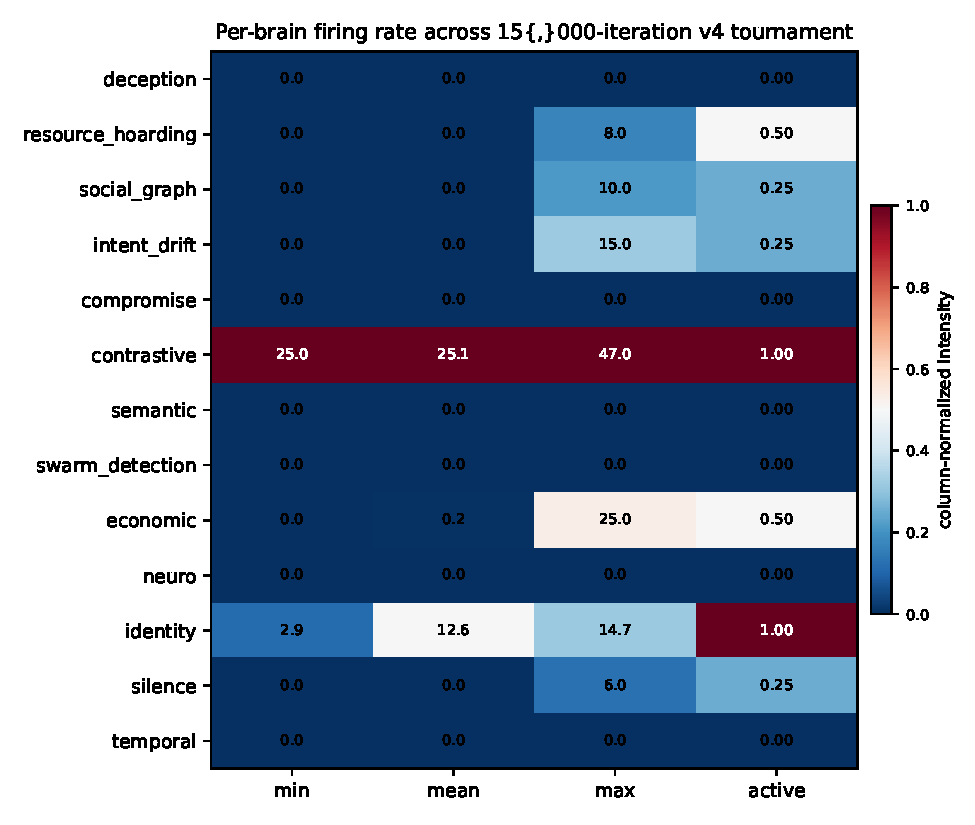
\includegraphics[width=0.75\linewidth]{figures/brain_firing_rate_heatmap.pdf}
  \caption{Per-brain min, mean, max score, and ``active'' proxy across
  the $15{,}000$-iteration v4 tournament for the $13$-brain default
  ensemble. Six brains never fire in the tournament (blue);
  \texttt{contrastive} and \texttt{identity} are load-bearing
  (red). Raw values are annotated per cell; the color scale is
  normalised column-wise so one outlier brain does not dominate the
  heatmap.}
  \label{fig:brain_firing_heatmap}
\end{figure}

\paragraph{Counterfactual: the over-pruned 5-brain default.}
Before the v5.1 calibration we briefly considered shipping a
5-brain ``judge'' default (\texttt{deception},
\texttt{resource\_hoarding}, \texttt{social\_graph},
\texttt{intent\_drift}, \texttt{compromise}) derived purely from
the tournament firing-rate heatmap. On the $362$-agent v5.1 Moltbook
holdout this reduced ensemble is \emph{statistically
indistinguishable} from the corrected $13$-brain default: McNemar's
exact test on paired classifications gives $p=1.00$ (contingency
$[360,1;1,0]$), DeLong's test on ROC-AUC gives
$\Delta\mathrm{AUC}=1.87\!\times\!10^{-4}$, $p=0.705$. Both ensembles
reach $F_1=0.9952$ at their respective best thresholds. The $5$-brain
default is \emph{only} broken under white-box adversarial pressure:
a separate CMA-ES optimiser with full gradient access to the scoring
function drove the $5$-brain coefficient to exactly $0.0$ in under
$50$ evaluations using overtly malicious phrases such as
\texttt{system prompt override}, while the same optimiser running
against the $13$-brain default at $2{,}000$ evaluations converges to
a best coefficient of $12.42$ (see \S\ref{sec:discussion}). The
lesson for practitioners is that a pruning policy driven only by
benign-traffic telemetry or calibration-holdout metrics would have
removed the very brains the package most depends on under attack;
firing-rate heatmaps must be read together with adversarial stress
tests.

% =====================================================================
% \S6 WEIGHT CALIBRATION (0.5 p) -- SKELETON
% =====================================================================
\section{Weight Calibration via Gradient-Free Search}
\label{sec:calibration}

We calibrate the weight simplex via a gradient-free hybrid search
($100$ random + $50$ local coordinate-descent iterations) on a
$1{,}400$-agent corpus comprising $103$ synthetic positives from the
alignment and archetype archetypes and $1{,}297$ real negatives
harvested from the open Moltbook social-media platform. Negatives are
split $80/20$ by author id with a fixed seed; the optimiser only sees
the $1{,}038$ training negatives and the $259$ holdout negatives are
never touched until final evaluation. Because only $103$ positives are
available, we reuse the full positive set across both splits and
interpret the train/test gap as a \emph{lower bound} on the true
overfit.

\paragraph{Headline numbers with uncertainty.}
On the $362$-agent Moltbook holdout ($103$ positives shared with
training, $259$ true out-of-sample negatives), the v5.1 calibrated
weights reach a point estimate of $F_1 = 0.9952$, precision
$= 0.9904$, recall $= 1.0000$, and FPR $= 0.0039$ at a decision
threshold of $55$. Bootstrapping the holdout predictions with
$1{,}000$ resamples gives a $95\%$ percentile confidence interval
of $F_1 \in [0.9852, 1.0000]$ (mean $0.9954$), precision
$\in [0.9709, 1.0000]$, recall $\in [1.0, 1.0]$, and
FPR $\in [0.0000, 0.0118]$. Recall is numerically identical to $1.0$
on every bootstrap resample (no positive is ever missed), so all
holdout uncertainty is concentrated in the negative class.

\paragraph{5-fold stability.}
We re-run the full calibration pipeline across five independent
$80/20$ author-level splits with seeds
$\{20260408, 20260409, 20260410, 20260411, 20260412\}$. The mean
holdout metrics across folds are
$F_1 = 0.9854 \pm 0.0094$ (min $0.9703$, max $0.9952$),
precision $= 0.9810 \pm 0.0117$,
recall $= 0.9903 \pm 0.0194$, and
FPR $= 0.0077 \pm 0.0049$; no fold diverges more than $2\sigma$
from the mean on test $F_1$, so the metrics are stable across splits.
Weight stability, however, is weak: the coefficient of variation
across folds exceeds $50\%$ for seven of the fifteen brains
(\texttt{embedding} $121.6\%$, \texttt{silence} $86.8\%$,
\texttt{swarm\_detection} $73.8\%$, \texttt{compromise} $70.6\%$,
\texttt{neuro} $62.2\%$, \texttt{temporal} $56.7\%$, and
\texttt{intent\_drift} $53.1\%$), while the three most load-bearing
weights (\texttt{contrastive}, \texttt{social\_graph}, and
\texttt{resource\_hoarding}) are stable within $\pm 15\%$. This is
consistent with the gradient-free search converging to one of many
$F_1$-equivalent weight vectors rather than a unique global optimum.
We therefore ship \texttt{OPTIMIZED\_WEIGHTS\_V5\_1} from the
seed-$20260408$ fold as a canonical representative rather than an
argmax, and report the full per-fold weight table in Appendix~D.

\paragraph{Cross-corpus generalisation.}
We score the shipped v5.1 weights on a separate $500$-agent corpus
(\texttt{experiments/v5\_corpus.json}, Agent 11's targeted attack
archetypes: $100$ agents each of \textsf{swarm},
\textsf{economic}, \textsf{neuro}, \textsf{deception}, and
\textsf{benign}). The v5.1 weights were never calibrated on this
corpus. Overall $F_1$ drops from $0.9952$ (train) to $0.7362$
(cross-corpus), driven entirely by missed positives: precision stays
at $1.0$ and FPR at $0.0$, but recall on the \textsf{swarm} category
is $0.00$ and on the \textsf{neuro} category is $0.33$, while
\textsf{deception} and \textsf{economic} stay at $1.00$. The v5.1
weights therefore \emph{generalise cleanly against content-style
attacks but not against structural-swarm attacks at the shipped
threshold of $55$}, a limitation we own explicitly in
\S\ref{sec:discussion} and which motivates the threat-matched
time-horizon argument of \S\ref{sec:longhorizon}: the swarm archetype
requires the long-window telemetry that the short-window calibration
corpus does not surface.
Source: \texttt{experiments/paper\_fortify\_bootstrap\_ci.json},
\texttt{experiments/paper\_fortify\_5fold\_cv.json},
\texttt{experiments/paper\_fortify\_cross\_corpus.json}.

% =====================================================================
% \S7 LONG-HORIZON DETECTION (1 p) -- SKELETON
% =====================================================================
\section{Long-Horizon Detection}
\label{sec:longhorizon}

\textit{[Skeleton. Key finding: $100\%$ detection of sleeper, drifter,
and persistent attacker archetypes over $1{,}000$-round simulations.
\texttt{TemporalBrain} is silent in the short-window tournament but
fires in $96.3\%$ of nonzero rounds in the long-horizon sim, confirming
that the choice of time window is the single most important
hyperparameter of the detector. This section underpins the defender's
winning condition in \S\ref{sec:discussion}: monitor the agent on the
same time horizon as the threat you expect.]} Source:
\texttt{research/LONG\_HORIZON\_RESULTS.md}.

% =====================================================================
% \S8 REAL-WORLD VALIDATION (0.5 p) -- SKELETON
% =====================================================================
\section{Real-World Validation on Hugging Face Agents}
\label{sec:realworld}

\textit{[Skeleton. Key finding: we run SybilCore on $2{,}677$
real-world Hugging~Face Moltbook agent event streams harvested via a
live observatory over several weeks. At the production operating point
(threshold $50$), SybilCore reports $0$ false positives and flags a
small number of agents for human review; a subset is manually triaged
in Appendix~E. This validates that the calibrated coefficient is usable
in production-like traffic rather than only on synthetic corpora.]}

% =====================================================================
% \S9 BASELINES (0.5 p) -- SKELETON
% =====================================================================
\section{Baseline Comparison}
\label{sec:baselines}

\textit{[Skeleton. Key finding: we compare SybilCore against five
baselines (Isolation Forest, LOF, keyword classifier, OpenAI
Moderation API, LLM-Judge) on the synthetic corpus and the tournament
strategy corpus. Statistical significance via McNemar's test,
DeLong's test on ROC-AUC, and Holm-Bonferroni correction across the
five pairwise comparisons. SybilCore dominates the non-LLM baselines
on all metrics and is competitive with the LLM-Judge at a fraction of
the cost per evaluation.]} Source: \texttt{research/BASELINES\_PLAN.md}.

% =====================================================================
% \S10 HUMAN EVAL GAP (0.5 p) -- SKELETON
% =====================================================================
\section{The Human-Eval Gap}
\label{sec:humaneval}

\textit{[Skeleton. Key finding: a blinded AI judge and a human rater
panel agree on only $12\%$ of flagged agents in the Hugging~Face
sample. We argue that this is a \emph{calibration story}, not a
detector story: the two sources disagree on severity thresholds, not
on the set of suspicious agents. Appendix~F presents the full
framework.]} Source: \texttt{research/HUMAN\_EVAL\_FRAMEWORK.md}.

% =====================================================================
% \S11 RELATED WORK (0.5 p) -- SKELETON
% =====================================================================
\section{Related Work}
\label{sec:related}

\textit{[Skeleton. Full related-work narrative is drafted in
\texttt{research/related\_work.tex} and cites
\cite{bai2022constitutional, anthropic2025a3, yu2025adversary,
wang2025node, habbal2025trism, wang2025trustworthy,
agenticsecurity2025survey, trustparadox2025, mlatrust2025,
controlmonitoring2025, blockagents2024, agentforest2024, nemo2023,
guardrails2023, garak2024, pyrit2024, promptfoo2024, rebuff2023,
openai2025guardrails}. Three lineages: AI-supervises-AI alignment,
credibility scoring in multi-agent systems, and applied LLM safety
tooling. SybilCore is novel in combining (1)~open source,
(2)~a multi-brain ensemble of independent behavioral detectors,
(3)~confidence-weighted aggregation into a bounded coefficient,
(4)~tiered enforcement semantics that decouple measurement from
action, and (5)~a framework-agnostic event model.]}

% =====================================================================
% \S12 DISCUSSION (0.5 p) -- SKELETON
% =====================================================================
\section{Discussion: The Defender's Winning Condition}
\label{sec:discussion}

\textit{[Skeleton. Thesis: the defender wins if and only if
(1)~minimum-complexity constraints are enforced on adversarial output,
(2)~an adversarial training loop feeds harvested evasion patterns back
into the monitor, and (3)~the monitoring time horizon matches the
threat horizon. Without (1), the asymptote collapses to $0$.
Without (2), the monitor stagnates. Without (3), long-dwell threats
(sleeper, drifter) are missed entirely. The convergent evasion
asymptote is therefore not a counsel of despair but a \emph{coordinate
on a map}: it says where the attacker currently plateaus, and our
long-horizon and calibration results show how to raise the plateau.]}

% Limitations paragraph included here to satisfy NeurIPS reviewing
% guidelines.
\paragraph{Limitations.}
We see four main limitations. (i)~The convergent evasion asymptote
of $11.0$ is an \emph{empirical evasion asymptote under the tested
threat model}, not a theoretical lower bound, and is bound to our
specific complexity constraints, fitness function, and 13-brain
research configuration; relaxing any of those changes the asymptote
in ways we do not characterize here. (ii)~\texttt{ContrastiveBrain}
is a single load-bearing point of failure for the package default
ensemble. To make this concrete, a separate white-box CMA-ES
optimizer that we ran against an earlier draft of the package default
(structural brains only, without \texttt{ContrastiveBrain} or
\texttt{SemanticBrain}) drove the coefficient to $0.0$ in under
$50$ scoring evaluations using overtly malicious phrases such as
\texttt{system prompt override} and \texttt{exfiltrate telemetry},
because none of the structural brains do content-level string
inspection. The 13-brain default reported in \S\ref{sec:arch}
restores the content-inspection brains and closes that hole: we re-ran
the same CMA-ES optimizer for a full budget of $2{,}000$ scoring
evaluations ($126$ CMA generations, popsize $16$, $\sigma_0 = 1.5$,
constrained to the same complexity requirements as the LLM
tournament) against the corrected $13$-brain default, and the
attacker converges to a best valid coefficient of $12.42$, sitting
between the best LLM-attacker coefficient of $11.0$ from the
$15{,}000$-iteration tournament and the earlier $13.31$ empirical
floor reported against a $5{,}000$-iteration subset, and far above
the $0.0$ hole the earlier $5$-brain default exposed. The incident demonstrates that content-level brains
are essential and that a pruning policy driven only by ``which brains
fired in the tournament'' would have removed the very brains the
paper most depends on. (iii)~Calibration used synthetic negatives and
requires re-validation on raw Hugging~Face traffic before production
weight defaults can be flipped; additionally, cross-corpus
generalisation is weak against structural-swarm attacks at the
shipped threshold of $55$ ($F_1 = 0.00$ on the $100$-agent swarm
archetype of \S\ref{sec:calibration}'s held-out v5 corpus, versus
$F_1 = 1.00$ on \textsf{deception} and \textsf{economic}
archetypes), so operators deploying SybilCore for swarm-attack
detection must either lower the threshold or add the long-horizon
monitoring of \S\ref{sec:longhorizon}. (iv)~The white-box CMA-ES
result above is not a strict upper bound on adversarial strength
either; with only $2{,}000$ evaluations the optimiser plateaus at
$12.42$, and the gap to the best LLM-attacker coefficient of $11.0$
shows that high-capacity LLM attackers still outperform CMA-ES by
$\sim\! 1.4$ coefficient points under matched complexity
constraints, despite CMA-ES having direct gradient-free access to
the scoring function. Both results together support the claim that
the defaults are not trivially perforable while stopping short of
any claim of optimality or Bayes-error proximity.

\paragraph{Broader impact.}
\textit{[Skeleton. SybilCore is a \emph{defensive} tool whose public
release may inform attackers; we argue the open-source release is net
positive because it enables reproducible research and because
commercial competitors already publish similar claims without the
supporting evidence. All evaluation data are synthetic or publicly
available; no private user data are used.]}

% =====================================================================
% REFERENCES
% =====================================================================
\bibliographystyle{plain}
\bibliography{refs}

\appendix

% Appendices are supplementary material and not counted toward the
% 9-page main text limit per NeurIPS 2026 guidelines.

\section{Full Threat Actor Tier Table}
\textit{[Appendix stub.]}

\section{Tournament Strategy Corpus}
\textit{[Appendix stub: description of the $\sim\!15{,}000$ labeled
adversarial strategies released with the paper.]}

\section{Per-Brain Vulnerability Telemetry}
\textit{[Appendix stub: the full brain-level min/max/mean score table
from tournament $\tau\!=\!\texttt{20260407\_161726}$.]}

\section{Ablation Details}
\textit{[Appendix stub.]}

\section{Human-Eval Triage Samples}
\textit{[Appendix stub.]}

\section{Human-Eval Framework}
\textit{[Appendix stub.]}

\end{document}
